\newpage
\section{Virtualizer}
\label{sec:virtualizer}
\hspace{\parindent}
One of the goals of the TSEngine was to use the motion platform Virtualizer Elite 2 available to robotic club. It is a device developed by Cyberith, capable of simulating endless space for the person to walk through. The Cyberith company provides SDK's for three languages, namely for C++, C\#, python, and two specially tailored ones for software development in C\# in Unity and in C++ in Unreal Engine. Using the device is quite simple and intuitive once you get familiar with it, and it is designed specially to use with a VR headset so as not to be limited by the space when immersing oneself in virtual reality. 
\begin{figure}[H]
  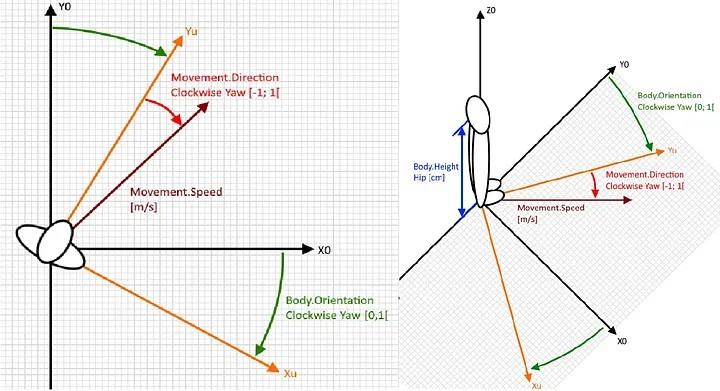
\includegraphics[width=\linewidth]{figures/cyberith_variables.jpg}
  \caption{Cyberith Virtualizer Elite 2 returned variables, image from Medium\cite{virtualizer_variables}}
\end{figure}
As one can see in the image above, the usage of virtualizer in practice comes down to handling four variables: body height, body orientation, movement speed and movement direction. Body height is measured in centimeters and can change if the ring of the Virtualizer is unlocked, allowing for recognition of crouching movement. Body orientation is measured on the hip height and is a value between zero and one, which represents the angle the Virtualizer's ring is turned. Movement speed is straightforward - it is measured in meters per second and depends on how fast the user moves their feet on the motion platform. Movement direction is  necessary to differentiate whether the user is moving forward or backwards.

Although the Virtualizer Elite 2 is designed for the virtual reality, it is completely viable to use it in different applications. One of the possible ideas of alternative use of the motion platform is to control the device like a robot remotely.
